\documentclass[12pt]{article}

\usepackage{a4wide}
\usepackage[utf8]{inputenc}

\usepackage{graphicx}
\usepackage{amsmath}
\usepackage{palatino}
\usepackage{url}

%\pagestyle{empty}

%\parindent=0pt
\begin{document}

\section*{Histogram of Oriented Gradients}

Object classification and detection is one of the major tasks in computer vision.
One of very successful methods is call Histogram of Oriented Gradients (HOG) \cite{dalal}.
It's a method that computes features for sought objects based on their gradients.
As you may guess, gradients are computed to form a histogram, based on which
objects are classified/detected.

\begin{figure}[h!]
    \center
    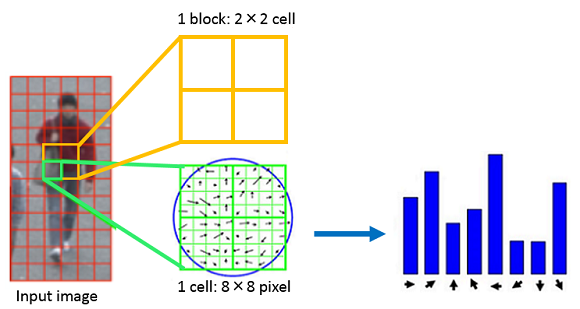
\includegraphics[width=0.9\textwidth]{hog_scheme.png}
    \caption{HOG Illustration \cite{img}}
    \label{fig:hog}
\end{figure}

\subsubsection*{Step 1: Compute the Gradient Image}

For each image pixel $(x, y)$, compute the orientation of gradient as
\begin{equation}
    \varphi(x,y) = \arctan \left( \frac{f_y(x,y)}{f_x(x,y)} \right) \,,
\end{equation}

and the size of gradient as

\begin{equation}
    e(x,y) = \sqrt{f_x^2(x,y) + f_y^2(x,y)} \,,
\end{equation}
where $f_x(x,y)$ and $f_y(x,y)$ are the differences of brightness in the $x$ and $y$ direction, respectively.
For their computing, we can use the following equations:
\begin{eqnarray}
    f_x(x,y) &= f(x+1,y) - f(x,y) \,, \\
    f_y(x,y) &= f(x,y+1) - f(x,y) \,.
\end{eqnarray}

\subsubsection*{Step 2: Create the Histograms}

Let the image be split into blocks of size $B_x \times B_y$, and let the blocks be split into cells of size $C_x \times C_y$ (see Fig. \ref{fig:hog}).
Create a histogram of gradient orientations in each cell.
Divide the range of orientations ($0-180$ or $0-360$ degrees) into $N$ bins (for example, with the step $20$ degrees that leads to $9$ bins for the interval $0-180$ degrees).
For each image pixel, add its gradient size into the bin representing the angle interval in which the gradient orientation of the pixel belongs.
Create such a histogram for each cell, and normalize the histograms within the blocks.

As a result of this method, we get a feature vector with the histogram values.
The size of the feature vector depends on the number of bins and on the number of cells in the image.
\newline
\newline

\begin{thebibliography}{2}
\bibitem{dalal}
Dalal, Navneet and Triggs, Bill: Histograms of Oriented Gradients for Human Detection, Proceedings of the 2005 IEEE Computer Society Conference on Computer Vision and Pattern Recognition (CVPR'05) - Volume 1, pp. 886--893,(2005)

\bibitem{img}
\url{http://www.lsi-contest.com/2017/shiyou_3-1e.html}
\end{thebibliography}

\end{document}
